%-- Add sections and your outline will be created automatically --%
\subsection{Rotating periodic channel}

% Frame starts a new slide
\begin{frame}
    \frametitle{Rotating periodic channel}
\begin{itemize}
\item Domain: Unit square, periodic in zonal direction and zero--slip at North and South boundaries and Coriolis forcing.
\item The flow is driven by a velocity source term:
\begin{equation*}
  \vec{F}=
  \begin{bmatrix}
    y^3 \\
    0
  \end{bmatrix}
\end{equation*}
\item Parameters are chosen such that the solution converges to a steady state with a known analytical solution.
\item A good example of using python state for online diagnostics and analysis, and also using python for setting initial conditions.
\end{itemize}
\end{frame}
%
\begin{frame}
    \frametitle{Rotating periodic channel}
\begin{figure}
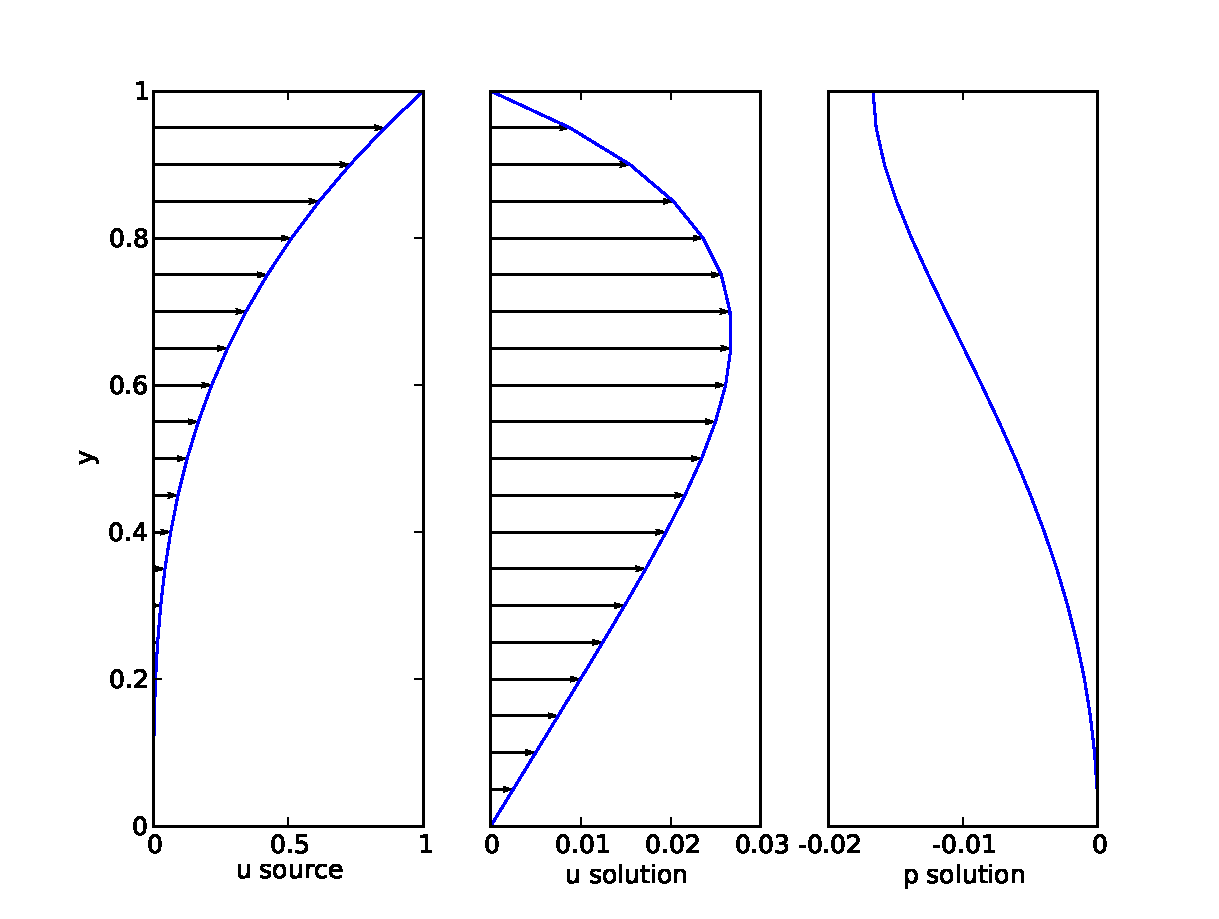
\includegraphics[width=0.6\textwidth]{./rotating_channel/analytic_solution}
\caption{Velocity forcing term and analytic solutions for velocity and pressure for the rotating periodic channel test case. Note that each of these quantities is constant in the x direction.}
\end{figure}
\end{frame}
%
\begin{frame}
    \frametitle{Rotating periodic channel}
\begin{figure}
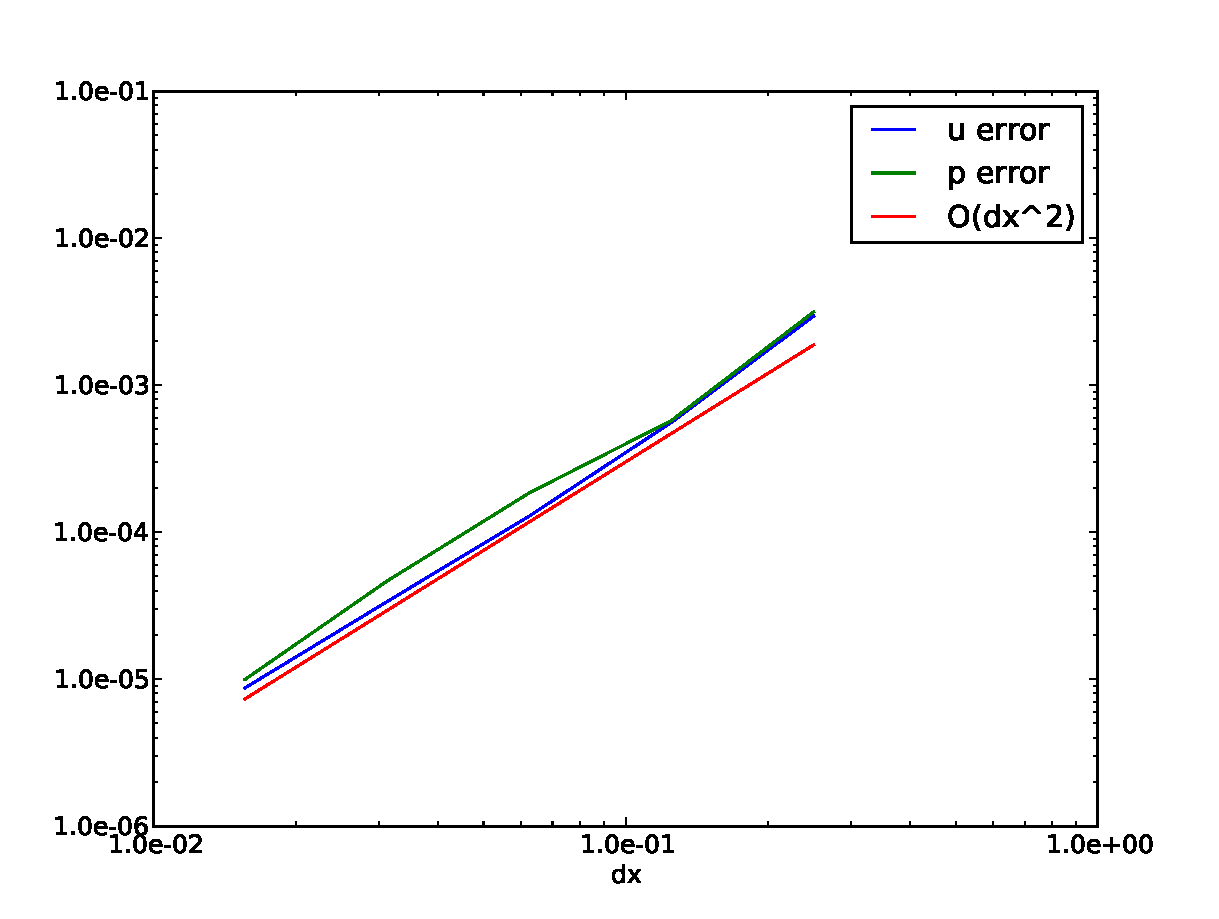
\includegraphics[width=0.6\textwidth]{./rotating_channel/convergence}
\caption{Error in the pressure and velocity solutions for the rotating channel as a function of resolution.}
\end{figure}
\end{frame}
%
\begin{frame}
    \frametitle{Rotating periodic channel, exercises}
\begin{itemize}
\item Understand the use of analytic forcing functions in Fluidity using Python.
\end{itemize}
\end{frame}

